\chapter{Referencial Teórico}

\section{Redes Sociais}

Quando se pensa em rede, surge a ideia de um conjunto de nós interligados entre si, como uma teia que ocupa um determinado espaço em um ambiente. Os nós ou pontos estão ligados em pares e podem representar várias situações em áreas de interesse em comum \cite{Newman:2010}.

Para Sodré \cite{Sodre:2002}, rede é onde as conexões e as interseções tomam o lugar do que seria antes apenas linearidade. Essas conexões e interações ocorrem pelo contato direto, face a face, e pelo contato indireto, utilizando-se um veículo mediador, como o telefone.

As redes sociais constituem uma das estratégias utilizadas pela sociedade para o compartilhamento da informação e do conhecimento, geralmente é formada mediante as relações entre indivíduos submetidos às mesmas pressões sociais ou que enfrentam idênticas dificuldades e obstáculos \cite{Tomae:Alcara:Chiara:2005}.

As pessoas estão inseridas na sociedade por meio das relações que desenvolvem durante toda sua vida, primeiro no âmbito familiar, em seguida na escola, na comunidade em que vivem e no trabalho; enfim, as relações que as pessoas desenvolvem e mantêm é que fortalecem a esfera social. A própria natureza humana nos liga a outras pessoas e estrutura a sociedade em rede \cite{Tomae:Alcara:Chiara:2005}.

Os tipos de relações também podem ser de movimentação entre lugares, como migração, mobilidade física ou social, conexão física, como uma estrada, um rio ou uma ponte que conecta dois lugares, de relações de autoridade ou relação biológica, como descendência, por exemplo \cite{Wasserman:1994}.

Com base em seu dinamismo, as redes, dentro do ambiente organizacional, funcionam como espaços para o compartilhamento de informação e do conhecimento. Espaços que podem ser tanto presenciais quanto virtuais, em que pessoas com os mesmos objetivos trocam experiências, criando bases e gerando informações relevantes para o setor em que atuam \cite{Tomae:Alcara:Chiara:2005}.

\begin{quote}
	``[...] na era da informação – na qual vivemos – as
	funções e processos sociais organizam-se cada vez
	mais em torno de redes. Quer se trate das grandes
	empresas, do mercado financeiro, dos meios de
	comunicação ou das novas ONGs globais,
	constatamos que a organização em rede tornou-se
	um fenômeno social importante e uma fonte crítica
	de poder.'' \cite{Capra:2002}
\end{quote}

O contexto em que estamos inseridos desencadeia uma série de mudanças na rotina dos indivíduos, e uma delas evidencia as redes como ponto de convergência da informação e do conhecimento \cite{Tomae:Alcara:Chiara:2005}.

O conhecimento que a rede possui repercute sobre o meio que esta se encontra, pois Wellman \cite{Wellman:1996} verifica, na rede, sua identidade singular em determinada situação, isto é, a representação e a interpretação das relações em rede estão fortemente ligadas à realidade que a cerca; a rede é influenciada pelo seu contexto e esse por ela.

Portanto os efeitos das redes podem ser percebidos fora de seu espaço, nas interações com o Estado, a sociedade ou outras instituições representativas \cite{Marteleto:2001}.

A interação constante ocasiona mudanças estruturais e, em relação às interações em que a troca é a informação, a mudança estrutural que pode ser percebida é a do conhecimento, quanto mais informação trocamos com o ambiente que nos cerca, com os atores da nossa rede, maior será nossa bagagem de conhecimento, maior será nosso estoque de informação, e é nesse poliedro de significados que inserimos as redes sociais \cite{Tomae:Alcara:Chiara:2005}.

Milgram, em sua tese \cite{Milgram:1967} defende que qualquer pessoa está distantes de qualquer outra pessoa do mundo, a no máximo seis graus de separação. Essa tese ficou conhecida como ``mundo pequeno'' e ``teoria dos seis degraus''. Sua pesquisa demonstra que a rede social constitui importante recurso profissional e pessoal. Estar em contato com pessoas que conheçam uma pessoa-alvo, em razão de um interesse específico, já é um passo além para a conquista de um objetivo.

\section{Teoria dos Grafos}

O desenvolvimento da análise de redes sociais tem como fundamento a teoria dos grafos, a seguir serão apresentados os principais conceitos sobre grafos.

\subsection{História}

O primeiro livro sobre a teoria dos grafos foi publicado por König (1936). Isso levou ao desenvolvimento de uma forte escola de teóricos em grafos na Hungria que incluíram P. Erdős e T. Gallai. Também na década de trinta, H. Whitney publicou uma série de artigos influentes \cite{Bondy:2007}.

De acordo com Ore \cite{Ore:1963}, Leonhard Euler\footnote{Grande matemático e físico suíço, 1707-1783, fez importantes descobertas em campos variados como Cálculo e Grafos.} teria sido um dos matemáticos mais importantes quando se refere a teoria dos grafos. Contam que o povo da cidade de Königsberg \footnote{atualmente Caliningrado.}, localizado na Prússia e cortada pelo Rio Pregel, com sete pontes ligando duas ilhas e as margens opostas do rio, como pode ser visto na Figura \ref{Konigsberg}, propôs ao então famoso matemático Leonard Euler o seguinte problema:

	“Será possível fazer um passeio pela cidade, começando e
	terminando no mesmo lugar, cruzando cada ponte exatamente uma vez?”

\begin{figure}[!h]
	\centering
	\includegraphics[scale=0.5]{figuras/capitulo2/Konigsberg.eps}
	\caption{Pontes de Königsberg}
	\label{Konigsberg}
\end{figure}

Não se sabe se Euler teria resolvido usando a representação de grafos que adotamos hoje. A modelagem do problema por grafo passa pela representação onde cada porção de terra  é representada por um ponto e as pontes estariam representadas por linhas \cite{Ore:1963}, apresentado na Figura \ref{sete_pontes}.

\begin{figure}[!h]
	\centering
	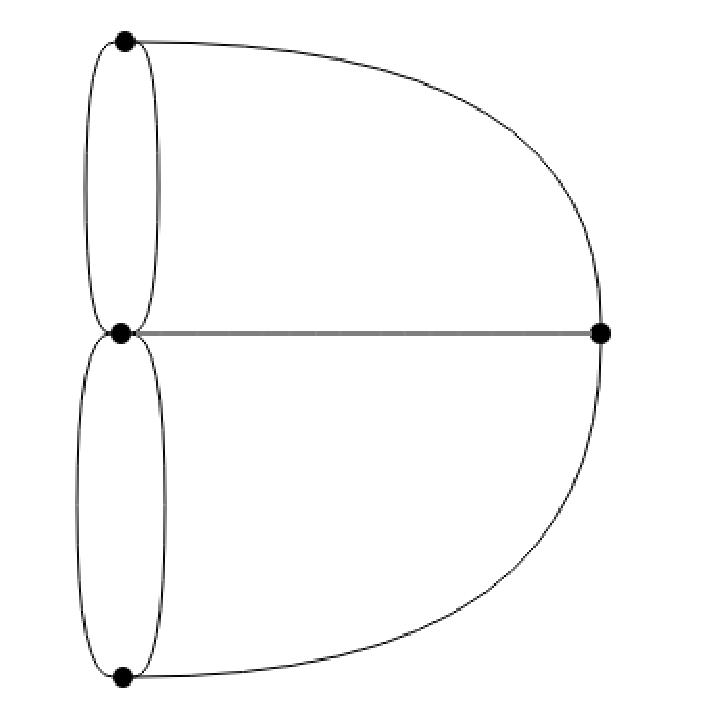
\includegraphics[scale=0.5]{figuras/capitulo2/sete_pontes.eps}
	\caption{Problema das sete pontes}
	\label{sete_pontes}
\end{figure}

Analisando, então, este grafo, Euler resolveu a questão provando que uma caminhada assim é possível se, e somente se, o grafo for conexo e todos os seus vértices tiverem grau par, termos estes que serão tratados mais à frente \cite{Malta:2008}.

Assim, Euler mostrou que, uma vez que o grafo de Königsberg tem vértices de grau ímpar, a resposta ao problema era que tal caminhada era impossível. Desde então todo grafo conexo cujos vértices possui grau par é chamado de grafo euleriano, e um caminho fechado em um grafo que passe por cada aresta deste exatamente uma vez é chamado de circuito (ou ciclo) euleriano \cite{Malta:2008}.

Graças à resolução dada por Euler, mais tarde muitos outros problemas importantes, para o desenvolvimento da Matemática Aplicada, foram possíveis de serem modelados. Dada a complexidade da vida nos grandes centros urbanos, muitos serviços precisaram ser organizados e é na Teoria de Grafos que encontramos uma modelagem para circuitos elétricos, rotas, distribuição de serviços (coleta de correspondências), coleta de lixo, distribuição de energia, água, luz, telefone \cite{Mello:2007}.

Também temos em Grafos a possibilidade de modelar relações de amizade, de hierarquia, de trabalho. Netto \cite{Netto:2012}, aponta grafos como um auxílio para o estudo de problemas envolvendo inter-relacionamento de elementos (em Química Orgânica, eletricidade, organização, transporte, psico-sociologia). Na verdade, grafos modelam diversas situações e muitas delas não quantificáveis.

Conforme Ore \cite{Ore:1963}, no século seguinte, o matemático irlandês William Hamilton \footnote{Nasceu em Dublin, na Irlanda, órfão de pai e mãe, especialista em línguas. Com dez anos falava razoavelmente uma meia dúzia de línguas orientais. Porém, aos 16 anos, demostrou interesse em matemática e decidiu se dedicar a sua vida a esta disciplina. Fazendo importantes contribuições.}, em 1859, inventou um jogo chamado ``\textit{The Icosian Game}'', com um peculiar enigma envolvendo um dodecaedro, em que cada um dos 20 vértices foram nomeados com nomes de cidades importantes. O objetivo do jogo era, utilizando as 30 arestas do dodecaedro, passar por cada uma das cidades apenas uma vez, começando e terminando na mesma cidade, um exemplo do grafo pode ser visualizado na Figura \ref{grafo_hamiltoniano}.

\begin{figure}[!h]
	\centering
	\includegraphics[scale=0.5]{figuras/capitulo2/grafo_hamiltoniano.eps}
	\caption{Grafo Hamiltoniano}
	\label{grafo_hamiltoniano}
\end{figure}

Apesar da simples formulação, o problema admite muitos caminhos como resposta. No problema de Hamilton temos uma diferença significativa em relação ao problema de Euler. Encontrar um caminho euleriano significa encontrar um caminho que passe por todas as arestas do grafo uma única vez, podendo ser aberto ou fechado. Nos caminhos hamiltonianos cada vértice é visitado uma única vez. O problema fica muito mais complexo com tal condição \cite{Costa:2011}.

\subsection{Definições}

\textbf{Definição 1}: Um grafo \textit{G} é um par ordenado \textit{(V(G), E(G))} que consiste de um conjunto \textit{V(G)} de vértices e um conjunto \textit{E(G)}, disjunto de \textit{V(G)}, de arestas, em conjunto com uma incidência função $\psi_G$ que associa a cada aresta de \textit{G} um par não ordenado de (não necessariamente distintas) vértices de \textit{G} \cite{Bondy:2007}.

\textbf{Definição 2}: Um grafo é um par \textit{G} = (\textit{V}, \textit{E}) de conjuntos de tal modo que \textit{E}$\subseteq$[\textit{V}$_2$]; Assim, os elementos de \textit{E} são subconjuntos de pares ordenados de elementos de \textit{V}. Para evitar ambiguidades de notação, deve-se sempre assumir tacitamente que \textit{V}$\cap$\textit{E}=$\oslash$. Os elementos de \textit{V} são os vértices (ou nós ou pontos) do grafo \textit{G}, os elementos de \textit{E} são arestas (ou linhas). A maneira usual de imaginar um grafo é pelo desenho de um ponto para cada vértice e juntando dois destes pontos por uma linha se os correspondentes dois vértices formam uma aresta. Assim como esses pontos e linhas são desenhadas é considerado irrelevante: o que importa é a informação de que pares de vértices formam uma aresta e quais não \cite{Diestel:1997}.

Grafos são assim chamados porque eles podem ser representada graficamente, e é esta representação gráfica que nos ajuda a entender muitas de suas propriedades. Cada vértice é indicado por um ponto, e de cada aresta por uma linha que une os pontos que representam as suas extremidades \cite{Bondy:2007}, um exemplo pode ser observado na Figura \ref{exemplo_grafo}.

\begin{figure}[!h]
	\centering
	\includegraphics[scale=0.5]{figuras/capitulo2/exemplo_grafo.eps}
	\caption{Exemplo de Grafo}
	\label{exemplo_grafo}
\end{figure}

A maioria das definições e conceitos na teoria dos grafos são sugeridas por esta representação gráfica. As extremidades de uma aresta são referidos como sendo incidente com a aresta, e vice-versa. Dois vértices que são incidente com uma aresta em comum são chamados de adjacentes e dois vértices adjacentes distintos são chamados de vizinhos \cite{Costa:2011}.

Uma aresta com extremidades idênticas é chamado um \textit{loop}, e uma aresta com extremidades distintas é um \textit{link}. Dois ou mais \textit{links} com o mesmo par de extremidades são referidos como sendo arestas paralelas \cite{Bondy:2007}. Na Figura \ref{loop_paralela} é possível observar a aresta ``a'' como uma aresta do tipo \textit{loop} e as aresta ``c'' e ``d'' como sendo arestas paralelas.

\begin{figure}[!h]
	\centering
	\includegraphics[scale=0.5]{figuras/capitulo2/loop_paralela.eps}
	\caption{Exemplo de loop e arestas paralelas}
	\label{loop_paralela}
\end{figure}

Um grafo é finito se tanto o seu conjunto de vértices, quanto o seu conjunto de arestas são finitos. Um grafo sem vértices (e, portanto, sem arestas) é o grafo nulo. Qualquer grafo apenas com um vértice é referido como trivial. Todos os outros grafos são não-triviais \cite{Costa:2011}.

Um grafo é simples se não tem \textit{loops} ou arestas paralelas \cite{Diestel:1997}, como exemplificado na Figura \ref{grafo_simples}.

\begin{figure}[!h]
	\centering
	\includegraphics[scale=0.5]{figuras/capitulo2/grafo_simples.eps}
	\caption{Exemplo de grafo simples}
	\label{grafo_simples}
\end{figure}

Certos tipos de grafos podem desempenhar papéis proeminentes na teoria dos grafos. Um grafo conexo é um grafo simples no qual quaisquer dois vértices são adjacentes, um grafo é vazio quando não há dois vértices adjacentes (isto é, o conjunto de arestas é vazio). Um grafo é bipartido se o seu conjunto de vértices pode ser particionado em dois subconjuntos \textit{X} e \textit{Y} para que cada aresta tem um fim em \textit{X} e um fim em \textit{Y}; uma tal partição (\textit{X}, \textit{Y}) é chamado uma bipartição do grafo, e \textit{X} e \textit{Y} suas partes. Pode-se denotar um grafo bipartido \textit{G} com bipartição (\textit{X}, \textit{Y}) por \textit{G}[\textit{X}, \textit{Y}]. Se \textit{G}[\textit{X}, \textit{Y}] é simples e todos os vértices de \textit{X} está associado a cada vértice em \textit{Y}, então \textit{G} é chamado de um grafo bipartido completo. Uma estrela é um grafo bipartido completo \textit{G}[\textit{X}, \textit{Y}] com |\textit{X}| = 1 ou |\textit{Y}| = 1 \cite{Diestel:1997}.  A Figura \ref{bipartido_completo} ilustra um grafo bipartido completo.

\begin{figure}[!h]
	\centering
	\includegraphics[scale=0.5]{figuras/capitulo2/bipartido_completo.eps}
	\caption{Grafo bipartido completo}
	\label{bipartido_completo}
\end{figure}

Um caminho é um grafo simples cujos vértices podem ser dispostos em uma sequência linear, de tal forma que dois vértices são adjacentes se forem consecutivos na sequência, e não adjacentes caso não forem consecutivos \cite{Bondy:2007}. Dessa forma, diz-se que um vértice é alcançável a partir de outro se houver um caminho levando o primeiro vértice ao último \cite{Costa:2011}.
(exemplo)

Do mesmo modo, um ciclo de três ou mais vértices é um grafo simples cujos vértices podem ser dispostos em uma sequência cíclica de tal maneira que dois vértices são adjacentes se forem consecutivos na sequência. Um ciclo em um vértice consiste de um único vértice com um ciclo, e um ciclo de dois vértices consiste em dois vértices ligados por um par de arestas paralelas. O comprimento de um caminho ou de um ciclo é o número de suas arestas \cite{Costa:2011}. É possível observar na Figura \ref{ciclos} alguns exemplos de grafos com ciclo.

\begin{figure}[!h]
	\centering
	\includegraphics[scale=0.5]{figuras/capitulo2/ciclos.eps}
	\caption{Exemplo de grafos com ciclos}
	\label{ciclos}
\end{figure}

Um grafo é conectado se, para cada partição de seus vértices definido em dois conjuntos \textit{X} e \textit{Y} não vazios, existe uma aresta com uma extremidade em \textit{X} e uma extremidade em \textit{Y}; caso contrário, o grafo é desconectado. Em outras palavras, um grafo é desconectado se a conjunto de vértices pode ser particionado em dois subconjuntos não vazios \textit{X} e \textit{Y} e que nenhuma aresta tem uma extremidade em \textit{X} e a outra extremidade em \textit{Y}, é instrutivo comparar esta definição com que de um grafo bipartido. Os exemplos de grafos conectados e desconectados são apresentados na Figura \ref{desconectados}, onde o grafo ``X'' e o grafo ``Y'' são dois grafos distintos conectados, porém se fossem trados como um único grafo este seria um grafo desconectado \cite{Bondy:2007}.

\begin{figure}[!h]
	\centering
	\includegraphics[scale=0.5]{figuras/capitulo2/desconectados.eps}
	\caption{Exemplo de grafos conectados e desconectados}
	\label{desconectados}
\end{figure}

\subsection{Representação de Grafos}

Embora desenhos são um meio conveniente de especificação de grafos, eles claramente não são adequado para armazenar grafos em computadores, ou para a aplicação de métodos matemáticos para estudar suas propriedades. Para estes fins, são consideradas duas matrizes associados com um grafo, uma matriz de incidência e uma matriz de adjacência \cite{Bondy:2007}.

Seja \textit{G} um grafo, com conjunto de vértices \textit{V} e conjunto de arestas \textit{E}. A matriz de incidência de \textit{G} é a matriz $M_G:= (m_{ve})$, com dimensões \textit{n$\times$m}, onde $m_{ve}$ é o número de vezes (0, 1, ou 2) que o vértice \textit{v} e aresta \textit{e} estão conectados \cite{Bondy:2007}.

A matriz de adjacência de \textit{G} é a matriz $A_G := (a_{uv})$, com dimensões \textit{n$\times$n}, em que uma $a_{uv}$ é o número de arestas que unem os vértices \textit{u} e \textit{v}, onde cada \textit{loop} conta como duas arestas. É possível verificar que a quantidade de memória necessária para essa representação é $\Theta(|\textit{V}|^2)$ \cite{Bondy:2007}. A Figura \ref{matriz} ilustra um grafo \textit{G} representado na matriz de incidência \textit{M} e na matriz de adjacência \textit{A}.

\begin{figure}[!h]
	\centering
	\includegraphics[scale=0.65]{figuras/capitulo2/matriz.eps}
	\caption{Representação em matriz}
	\label{matriz}
\end{figure}

Pela maioria dos grafos possuírem um número bem maior de arestas do que os vértices, a matriz de adjacência de um grafo geralmente é menor do que a sua matriz de incidência e, assim, necessita de menos espaço de armazenamento. Ao lidar com grafos simples, uma representação ainda mais compacto é possível. Para cada vértice \textit{v}, os vizinhos de \textit{v} são armazenados em uma lista. A lista (\textit{N}(\textit{v}): \textit{v $\in$ V}) é chamada de lista de adjacência do grafo, onde \textit{N}(\textit{v}) representa a os vizinhos do vértice \textit{v}, um exemplo pode ser observado na Figura \ref{lista_adjacencia}. A quantidade de memória necessária para uma lista de adjacências é $\Theta(|\textit{V}| + |\textit{E}|)$. Grafos simples são normalmente armazenados em computadores como listas de adjacência \cite{Costa:2011}.

\begin{figure}[!h]
	\centering
	\includegraphics[scale=0.5]{figuras/capitulo2/lista_adjacencia.eps}
	\caption{Representação em lista de adjacência}
	\label{lista_adjacencia}
\end{figure}

O grau de um vértice \textit{v} em um grafo \textit{G}, designado por \textit{d$_G$}(\textit{v}) é o número de arestas de \textit{G} que incidem em \textit{v}, para cada \textit{loop} é contado duas arestas. Em particular, se \textit{G} é um grafo simples, \textit{d$_G$}(\textit{v}) é o número de vizinhos de \textit{v} em \textit{G}. Um vértice de grau zero é chamado um vértice isolado. Denominamos por $\delta$(\textit{G}) e $\Delta$(\textit{G}) mínimo e máximo graus dos vértices de \textit{G}, e por \textit{d}(\textit{G}), o seu grau médio, $\frac{1}{n}\sum_{\textit{v}\in\textit{V}} \textit{d}(\textit{v})$ \cite{Diestel:1997}.

Embora muitos problemas possuem formulação na da teoria dos grafos, o conceito de um grafo, por vezes, não é suficientemente adequado. Ao lidar com problemas de fluxo de tráfego, por exemplo, é necessário saber quais estradas são de sentido único e em quais é permitido o tráfego nos dois sentidos. Para contextualizar esse problema é preciso um grafo em que cada ligação tem uma orientação atribuída, ou seja, um grafo dirigido \cite{Bondy:2007}. Um exemplo de grafo dirigido pode ser observado na Figura \ref{dirigido}.

\begin{figure}[!h]
	\centering
	\includegraphics[scale=0.5]{figuras/capitulo2/dirigido.eps}
	\caption{Exemplo de grafo dirigido}
	\label{dirigido}
\end{figure}

Formalmente, um grafo dirigido \textit{D} é um par ordenado \textit{(V(D), E(A))} que consiste de um conjunto \textit{V(G)} de vértices e um conjunto \textit{A(G)}, disjunto de \textit{V(G)}, de arcos, em conjunto com uma incidência função $\psi_D$ que associa a cada arco de \textit{D} um par ordenado de (não necessariamente distintas) vértices de \textit{D}. Se \textit{a} é um arco e $\psi_D$(\textit{a}) = (\textit{u,v}), então \textit{a} é dito como como a junção de \textit{u} para \textit{v}, pode-se dizer que \textit{u} domina \textit{v} \cite{Diestel:1997}.

\subsection{Árvores e Florestas}

Um grafo acíclico é aquele que não contém ciclos. Um grafo acíclico conectado é chamado de uma árvore. As árvores em seis vértices estão apresentados na Figura \ref{arvores_seis_vertices}. De acordo com estas definições, cada componente de um gráfico acíclico é uma árvore. Por esta razão, gráficos acíclicos são geralmente chamados florestas \cite{Bondy:2007}.

\begin{figure}[!h]
	\centering
	\includegraphics[scale=0.5]{figuras/capitulo1/arvores_seis_vertices.eps}
	\caption{Exemplo de árvores com seis vértices}
	\label{arvores_seis_vertices}
\end{figure}

Em uma árvore, quaisquer dois vértices são conectados por exactamente um caminho. E Diestel \cite{Diestel:1997}, representa esse único caminho de ligação vértices \textit{x} e \textit{y} em uma árvore \textit{T} por \textit{xTy}.

Uma árvore com raiz \textit{T}(\textit{x}) é uma árvore \textit{T} com um vértice específico \textit{x}, chamado a raiz de \textit{T}. Uma orientação de uma árvore com raiz, todos vértices, excluindo o vértice raiz \textit{x}, é chamado de ramificação \cite{Bondy:2007}. Um exemplo de uma árvore com raiz pode ser obeservado na Figura \ref{arvore_raiz}.

\begin{figure}[!h]
	\centering
	\includegraphics[scale=0.3]{figuras/capitulo1/arvore_raiz.eps}
	\caption{Exemplo de uma árvore com raiz}
	\label{arvore_raiz}
\end{figure}

\section{Algoritmos}

\subsection{Busca em Grafos}

A busca em grafos refere-se ao método de explorar o grafo, ou seja, obter um método sistemático para percorrer seus vértices e arestas. Para isto, há dois principais algoritmos, busca em profundidade (\textit{DFS - Depth First Search}) e busca em largura (\textit{BFS - Breadth First Search}). Em ambos os casos parte-se de um vértice qualquer.

\subsubsection{DFS}
A ideia por trás do \textit{DFS} é alcançar ``mais fundo'' no grafo quando possível. A ordem em que os vértices são visitados depende da ordem em que os vizinhos de cada vértice aparecem na lista de adjacência \cite{Cormen:2001}. Considere as figuras a seguir para a exemplificação do DFS.

\begin{figure}[!h]
	\centering
	\includegraphics[scale=0.4]{figuras/capitulo1/dfs/dfs1.eps}
	\caption{Exemplo DFS etapa 1}
	\label{dfs1}
\end{figure}

A busca irá partir do vértice arbitrátio \textit{v}, chamado de vértice raiz. A partir do vértice raiz é possível percorrer três arestas: (\textit{v}, \textit{a}), (\textit{v}, \textit{b}) e (\textit{v}, \textit{c}). A aresta a ser seguida será (\textit{v}, \textit{a}).

\begin{figure}[!h]
	\centering
	\includegraphics[scale=0.4]{figuras/capitulo1/dfs/dfs2.eps}
	\caption{Exemplo DFS etapa 2}
	\label{dfs2}
\end{figure}

O vértice \textit{a} possui três arestas, que são: (\textit{a}, \textit{v}), (\textit{a}, \textit{b}) e (\textit{a}, \textit{d}). Como o vértice \textit{v} já foi visitado, a aresta a ser seguida será (\textit{a}, \textit{b}).

\begin{figure}[!h]
	\centering
	\includegraphics[scale=0.4]{figuras/capitulo1/dfs/dfs3.eps}
	\caption{Exemplo DFS etapa 3}
	\label{dfs3}
\end{figure}

A partir de \textit{b} é possível escolher as seguintes arestas: (\textit{b}, \textit{v}), (\textit{b}, \textit{a}) e (\textit{b}, \textit{c}), porém como os vértices \textit{v} e \textit{a} já foram visitados, a opção restante será a aresta (\textit{b}, \textit{c}).

\begin{figure}[!h]
	\centering
	\includegraphics[scale=0.4]{figuras/capitulo1/dfs/dfs4.eps}
	\caption{Exemplo DFS etapa 4}
	\label{dfs4}
\end{figure}

Ao alcançar \textit{c}, há duas possibilidades: (\textit{c}, \textit{v}) e (\textit{c}, \textit{b}), porém ambos os vérices \textit{v} e \textit{b} já são conhecidos, então não há para onde se aprofundar, entretando ainda existem vértices não descobertos. Nesse caso deve-se voltar até o vértice \textit{b}, verificando se há alguma aresta que leva a um vértice ainda não visitado. No caso não há, então volta-se novamente pelo caminho percorrido, chegando ao vértice \textit{a}. Em \textit{a}, a aresta (\textit{a}, \textit{d}) leva a um vértice ainda não descoberto, portanto esse caminho deve ser tomado.

\begin{figure}[!h]
	\centering
	\includegraphics[scale=0.4]{figuras/capitulo1/dfs/dfs5.eps}
	\caption{Exemplo DFS etapa 5}
	\label{dfs5}
\end{figure}

Em \textit{d} há dois caminhos a seguir: (\textit{d}, \textit{a}) e (\textit{d}, \textit{e}), porém a única aresta que leva a um vértice não visitado é (\textit{d}, \textit{e}), portanto esta deverá ser seguinda.

\begin{figure}[!h]
	\centering
	\includegraphics[scale=0.4]{figuras/capitulo1/dfs/dfs6.eps}
	\caption{Exemplo DFS etapa 6}
	\label{dfs6}
\end{figure}

Ao alcançar o vértice \textit{e}, todos os vértice foram visitados, portanto o percuso realizado pelo \textit{DFS} pode ser observado na Figura \ref{dfs_percurso}, e que é uma árvore.

\begin{figure}[!h]
	\centering
	\includegraphics[scale=0.4]{figuras/capitulo1/dfs/dfs_percurso.eps}
	\caption{Percurso do DFS}
	\label{dfs_percurso}
\end{figure}

O algoritmo para a busca em profundidade pode ser visualizado no algoritmo a seguir. Nele, \textit{prework} e \textit{postwork} dependem da aplicação do DFS, definindo as ações que devem ser tomadas, respectivamente, quando um vértice é marcado e quando é necessário voltar por uma aresta ou quando a aresta leva a um vértice já visitado \cite{Manber:1989}.

\begin{lstlisting}[language=Ada]
Algoritmo DFS(G,v):
Entrada: G = (V,E), um grafo nao dirigido, e v pertece a V .
Saida: depende da aplicacao.

inicio
	marque v;
	execute prework em v;
	para todas as arestas (v, w) faca
		se w nao estiver marcado entao DFS(G,w);
		execute postwork para (v, w);
fim
\end{lstlisting}

Caso o grafo seja conexo, então todos os seus vértices serão marcados pelo algoritmo anterior, e todas as suas
arestas serão visitadas pelo menos uma vez durante a execução do algoritmo \cite{Manber:1989}.

\subsubsection{BFS}

\subsection{Ordenação Topológica}

\subsection{Caminhos Mais Curtos}

\subsubsection{Algoritmo de Dijkstra}

\subsection{Árvore Geradora Mínima}

\subsection{Fluxo em Rede}

\section{Reutilização de Software}

A reutilização de software tem como objetivos aumentar a qualidade e produtividade no desenvolvimento, pois busca evitar duplicidade de código e do esforço aplicado para desenvolver determinadas tarefas e reaproveita o máximo possível experiências passadas \cite{Lucredio:2009}.

Todas as formas de reutilização de software usam algum tipo de abstração.  Essa é uma característica importante presente nas técnicas de reutilização, pois facilita aos desenvolvedores o uso. Sem abstrações os desenvolvedores deveriam analizar todos os artefatos reutilizáveis buscando entender como cada um funciona e como e quando devem ser utilizados \cite{Krueger:1992}.

Os próximos sub-tópicos irão apresentar temas deste trabalho que estão diretamente relacionados a reutilização de software.

\subsection{Frameworks}

Frameworks compartilham técnicas de reutilização em geral e são considerados uma importante parte da cultura de desenvolvimento no mundo da orientação a objetos \cite{Johnson:1997}.

Fayad e Schimidt em seu artigo \cite{Fayad:Schimidt:1997} sobre frameworks de aplicações orientadas a objetos mostram quais são os principais benefícios no uso de frameworks, que são: modularização, reutilização, extensibilidade e inversão de controle.

\begin{itemize}
	\item \textbf{Modularização:} Frameworks encapsulam e interfaceiam alguns detalhes de implementação, isso reduz o esforço necessário para entender e manter partes do software existente, pois basta ao desenvolvedor usar o que lhe é oferecido sem necessariamente entender qual a implementação do framework.

	\item \textbf{Reutilização:} As interfaces providas por frameworks ajudam também na reutilização através da definição de componentes genéricos, que podem ser aplicadas em outras aplicações. Dessa forma, soluções comuns para sistemas diferentes podem ser usadas da mesma forma sem a necessidade de recriação das mesmas. Entende-se então, que estas soluções são pensadas uma única vez e ao estarem presentes em um framework basta que sejam usadas.

	\item \textbf{Extensibilidade:} Este é um dos principais pontos positivos dos frameworks, pois os frameworks fornecem métodos e interfaces estáveis que outras aplicações irão utilizar, e essas aplicações devem poder usar esses métodos visando resolver problemas parecidos em diferentes contextos. Uma boa estrutura de extensibilidade é essencial para garantir a customização de novos serviços e funcionalidades das aplicações.

	\item \textbf{Inversão de controle:} A inversão de controle ocorre devido a forma como serão processados e entendidos muitos dos eventos de uma aplicação, que ficam invisíveis ao desenvolvedor quando este usa um framework, pois é o próprio framework quem decide o conjunto de métodos que será invocado para realizar uma determinada tarefa da aplicação.
\end{itemize}

\subsubsection{Frameworks e Reutilização de Software}

A tecnologia de reutilização ideal provê componentes que podem facilmente ser conectados para criar um novo sistema. Não é necessário ao desenvolvedor ter conhecimento de como o componente é implementado e geralmente é fácil para ele aprender como o utilizar. O resultado é que o sistema será eficiente, fácil de manter e confiável \cite{Johnson:1997}.

Frameworks são aplicações especializadas em prover classes e componentes abstratos que podem ser usados por outros sistemas. Estes proveem técnicas de reutilização resistentes e de maior granularidade. Sendo aplicações independentes é mais fácil usá-los em um maior número de sistemas \cite{Johnson:Foote:1988}.

Para se alcançar a aplicação efetiva de um dado framework é necessário ao desenvolvedor conhecer as interfaces que o framework proporciona antes de poder usá-las. Como podem existir diversas interfaces complexas aprender a usar um novo framework pode ser difícil. Porém, os frameworks são poderosos e o tempo gasto em sua aprendizagem é recompensado, pois podem reduzir a quantidade de esforço aplicado para se desenvolver uma nova aplicação que os usem \cite{Johnson:1997}.

Ao longo do tempo tornou-se muito caro desenvolver aplicações complexas a partir do zero. Isso porque todos os componentes que são desenvolvidos devem passar por um criterioso processo de validação e manutenção e isso ocorre sempre que um novo sistema é desenvolvido. Ao se usar frameworks pode-se desenvolver componentes comuns e os processos citados são feitos em um único local \cite{Fayad:Schimidt:1997}.

As técnicas de reutilização são diferentes de acordo como o tipo do framework utilizado, esses tipos podem ser ``\textit{white box}'' ou ``\textit{black box}''. O primeiro diz respeito a quando o código do framework é aberto e visível ao desenvolvedor, dessa forma, este pode estudar a implementação do framework e modificar o código de determinadas partes de acordo com suas necessidades. Os frameworks do tipo ``\textit{black box}'' disponibilizam apenas interfaces ao desenvolvedor para que este possa usá-las, a forma como tudo é implementado e processado é desconhecida. No primeiro tipo têm-se uma maior flexibilidade, porém, o uso é mais complexo ao desenvolvedor. No segundo o uso é bem simples, porém, não existe flexibilidade para mudança da implementação \cite{Kroth:2000}.

Além dos tipos de frameworks, estes também podem ser divididos quanto a sua aplicabilidade. Podem ser desenvolvidos para serem aplicados em qualquer domínio, de forma genérica sem se preocupar com algo específico \textit{frameworks horizontais}, ou podem ser desenvolvidos visando atender um tipo específico de domínio de problemas, \textit{frameworks verticais}, essas caracteríscas dependem das necessidades apresentadas ao se trabalhar com frameworks e isso impacta como será aplicada a reutilização \cite{Kroth:2000}.

Na Engenharia de Software busca-se cada vez mais o aumento da produtividade e da qualidade dos sistemas desenvolvidos. A reutilização de software, ao contrário de todas as outras partes de um sistema é um fator que pode acarretar o aumento desses fatores, considerando que ao se utilizar componentes já desenvolvidos e depurados pode-se reduzir o tempo de desenvolvimento, de testes e as chances de ocorrência de erros que poderiam advir se fosse necessário a criação destes novos artefatos \cite{Silva:2000}.

Além de ganhos na produtividade e na qualidade a reutilização advinda dos frameworks pode trazer ganhos de desempenho, confiabilidade e interoperabilidade de software \cite{Fayad:Schimidt:1997}.

\subsubsection{Frameworks e Padrões}

Padrões representam soluções recorrentes para problemas no desenvolvimento de software em um contexto específico. Tanto os padrões como os frameworks são técnicas de reutilização, a grande diferença é que os frameworks 	se concentram na reutilização de estruturas, algoritmos e implementações em uma dada linguagem de programação, já os padrões focam em apresentar desenhos abstratos de como resolver problemas, são como microarquiteturas de software \cite{Fayad:Schimidt:1997}.

Um padrão descreve um problema a ser resolvido e apresenta uma solução e o contexto em que essa solução funciona, nomeia uma técnica e descreve seus custos e benefícios \cite{Johnson:1997}.

Quando um framework é implementado diversas vezes este também pode ser considerado um padrão. O MVC\footnote{http://www.dsc.ufcg.edu.br/$\sim$jacques/cursos/map/html/arqu/mvc/mvc.htm} (\textit{Model / View / Controller}) é um framework de interface com usuário que é considerado um padrão \cite{Johnson:1997}.

Quando usados em conjunto com padrões os frameworks podem aumentar significativamente a qualidade do software e reduzir o esforço de desenvolvimento \cite{Fayad:Schimidt:1997}.

\subsection{Padrões de Projeto}

Os padrões de Projeto são parte da vanguarda da tecnologia orientada a objetos e este tema tem estado em constante crescimento no decorrer dos tempos. A proposição por trás dos padrões é que a qualidade do software pode ser medida objetivamente, isso considera que ao se analisar o design de um padrão este pode ser considerado bom ou ruim, e assim resultando em uma boa ou má qualidade \cite{Shalloway:Trott:2004}.

Alexander em seu livro \cite{Alexander:1979} sobre padrões de construção diz:

\begin{quote}
	``cada padrão descreve um problema no nosso
ambiente e o cerne da sua solução, de tal forma que você possa usar essa solução mais
de um milhão de vezes, sem nunca fazê-lo da mesma maneira''
\end{quote}

No livro de padrões de projeto \cite{Gamma:Helm:Johnson:Vlissides:1995} o autor concorda com as afirmações de Alexander, a diferença principal é que no âmbito de software os padrões são expressos em termos de objetos e interfaces ao invés de paredes e portas, porém, em ambos os tipos os padrões dizem respeito a uma solução para um problema em um contexto geral. Além disso Gamma considera que um padrão é dividido em quatro partes principais que são:

\begin{itemize}
	\item \textbf{Nome:} Usado para descrever um problema de projeto, suas soluções e consequências em uma ou duas palavras. Quando um padrão possui um nome fica mais fácil de definir um vocabulário comum para tratar deste com outras pessoas.
	\item \textbf{Problema:} O problema está ligado diretamente a situação em que deve ser aplicado o padrão, ou seja, qual o contexto. Algumas vezes o problema pode conter uma lista de condições que devem ser satisfeitas para que se possa alcançar sentido na aplicação do padrão.
	\item \textbf{Solução:} Esta descreve todos os elementos que compõem o padrão, seus relacionamentos, responsabilidades e colaborações. É fornecida uma descrição abstrata de um problema de projeto e o arranjo geral de classes e objetos que resolvam o padrão, não há uma solução ou implementação concreta pois padrões são desenhados para serem usados em muitas situações diferentes.
	\item \textbf{Consequências:} As consequências apresentam uma série de resultados concernentes da aplicação do padrão, devem ser apresentadas vantagens e desvantagens. São elementos críticos que entram na decisam da aplicação ou não do padrão que está em questão.
\end{itemize}

\subsubsection{Por que usar Padrões de Projeto?}

Os dois pontos que melhor justificam o uso de Padrões de Projeto são porque estes são soluções reutilizáveis e estabelecem uma terminologia comum de acordo com \cite{Shalloway:Trott:2004}. A seguir há uma breve descrição de cada um de acordo com os autores mencionados.

\begin{itemize}
	\item \textbf{Soluções Reutilizáveis:} O tempo gasto para aprender a utilizar determinado padrão vale a pena pela reutilização que é oferecida. Têm-se o benefício de aplicar o que foi aprendido para diversos projetos e depois de ter o conhecimento fixado não é necessário reinventar soluções para problmeas recorrentes, basta reutilizar o que os padrões oferecem.
	\item \textbf{Terminologia Comum:} Quando se está em um grupo de trabalho é necessário uma base de vocabulário e pontos de visão do problema comuns. Os padrões de projeto providenciam um ponto comum de referência durante as fases de analise e design de um projeto.
\end{itemize}

Além do que já foi citado, diz o autor que os padrões dão aos desenvolvedores uma perspectiva de alto nível do problema a ser resolvido, isso facilita o entendimento do problema e uma melhor elaboração de solução.

Gamma ainda diz que os padrões podem ajudar na refatoração de projetos. Um das grandes dificuldades no desenvolvimento de software é que este tem de ser frequentemente reorganizado ou refatorado, os padrões de projeto ao oferecerem soluções comuns e já consolidadas podem reduzir a quantidade de refatoração que deverá ser feita mais tarde \cite{Gamma:Helm:Johnson:Vlissides:1995}.

A figura \ref{ciclo de vida oo} representa o ciclo de vida de aplicações orientadas a objeto segundo \cite{Gamma:Helm:Johnson:Vlissides:1995}.

\begin{figure}[!h]
	\centering
	\includegraphics[scale=0.5]{figuras/capitulo2/ciclo_de_vida_oo.eps}
	\caption{Ciclo de vida de aplicações orientadas a objetos}
	\label{ciclo de vida oo}
\end{figure}

A prototipação consiste da vida inicial do software que consiste de um conjunto inicial de requisitos. Normalmente nessa etapa são criadas as classes de domínio que representam as entidades principais do domínio inicial do problema.

Após a etapa de prototipação entra-se na etapa de ``mais requisitos'' e começa-se uma expanção para atender esses novos requisitos, porém, esta fase deve ser pensada cautelosamente e não pode ser longa pois o software pode acabar se tornando muito inflexível, é aí que entra a etapa de ``reutilização'' que pode ser definida por um processo de refatoração onde busca-se separar componentes de finalidades genéricas visando alcançar partes retilizáveis para o sistema em desenvolvimento.

Por fim, têm-se a etapa de consolidação onde se obtêm um software mais genérico e que atenda mais requisitos.

Esse é um ciclo inevitável e quando se pensa desde o início em refatorações futuras que podem vir a ser necessárias busca-se a aplicação de padrões que podem evitar tais refatorações \cite{Gamma:Helm:Johnson:Vlissides:1995}.

\subsubsection{Os Padrões de Projeto}

No livro de Padrões de Projeto foram definidos e classificados 23 padrões essa classificação está feita de acordo com dois critérios: \textbf{finalidade} e \textbf{escopo}. O primeiro critério diz respeito ao que o padrão faz, a finalidade pode ser de criação, estrutural ou comportamental. Os padrões de finalidade de criação se preocupam com o processo de criação de objetos, os estruturais focam em composições, de classes ou objetos e os comportamentais caracterizam as maneiras que as classes ou objetos interagem e distribuem responsabilidades.

O segundo critério especifica se o padrão é de classe ou objeto. Os padrões de classes lidam com relacionamentos entre classes e suas subclasses, para isso usa-se relacionamentos de herança e os padrões de objetos são mais dinâmnicos pois lidam com relacionamentos entre objetos que podem ser mudados em tempo de execução.

A tabela \ref{divisao dos padroes} ilustra a divisão dos padrões entre finalidade e escopo \cite{Gamma:Helm:Johnson:Vlissides:1995}.

AINDA FALTA A TABELA.

\subsection{Software com Serviço}
